% Drawing 154/03-8 -- folder 154, batch 03, archive page 56 (PDF page 57).
% Transcription: deux autres écuelles, l'une marquée $-1$ de part et d'autre, suivie de « $\ldots$ », et de nouveau « $(3, 3)$ $(3, 4)$ --- » à l'envers ; un cercle vert et noir avec des arcs épais noirs et des marques rouges, annoté $1/2$, $1/1$, $1$ ; en haut à droite, un pentagone aux sommets numérotés $0$ à $3$ et un quadrilatère, avec « $1\,2\,3$ » ; au bas, trois grands cercles au crayon, avec des arcs épais noirs et des points verts, l'un marqué $+$ en haut
% Kind: bowls, circles with thick arcs, polygons (several figures). Method 2 (schematic redraw from the facsimile). Status: partial.
% Notes: Several figures over a printed listing (CRAY2 job banner, 17 Aug 82, typed notice; not reproduced), read from the page view. Two more « bowls » (the first marked -1 on both sides), the upside-down « (3,3) (3,4) --- » above them; a green and black circle with thick black arcs and red marks, annotated 1/2, 1/1, 1 (positions of the fractions approximate); top right a pentagon with vertices numbered 0 to 3 and a quadrilateral, with « 1 2 3 »; at the foot three large pencil circles with thick black arcs and green points, the middle one marked + at the top and holding an inner lens. The three bowls at the top centre of the page precede this mark and are not covered by it. The polygons at the top right are small and partly cut by the torn corner; their numbering is placed, not all read.
% Coordinates: 1 unit = 1 mm = 1/100 of the crop width (bbox in page fractions: [0.193, 0.069, 0.927, 0.515]).
% Redrawn by Claude (claude-opus-5-5), issue #73, 2026-11-07; not checked by a human; not compiled (no TeX in the session).
% Rights: reproduces part of the work -- behind RENDER_TRANSCRIPTS, never published by itself.
\documentclass[tikz,border=3pt]{standalone}
\usepackage{amsmath,amssymb}
\usetikzlibrary{patterns,arrows.meta}
\tikzset{Or/.style={orange!90!black}, Ye/.style={yellow!80!orange}, Lg/.style={green!60!black!70}, Dg/.style={green!45!black}, Br/.style={brown!80!black}, Rd/.style={red!85!black}, Bl/.style={blue!70!black}, Gy/.style={black!40}, pencil/.style={black!45}, struck/.style={black!35}, mark/.style={circle,draw,inner sep=1.3pt}, pt/.style={circle,fill,inner sep=0.9pt}, opt/.style={circle,draw,fill=white,inner sep=1.1pt}}
\begin{document}
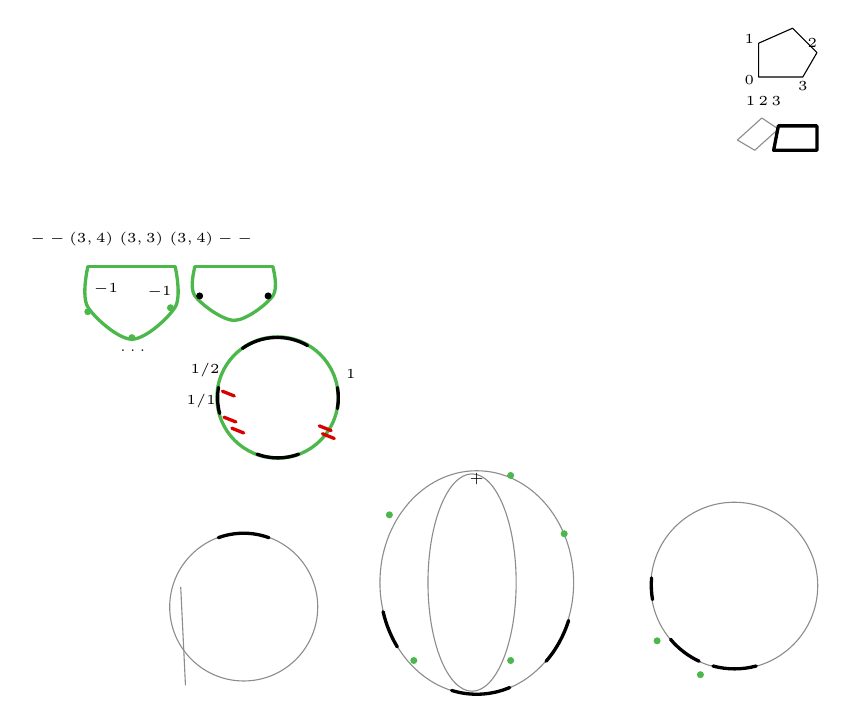
\begin{tikzpicture}[x=1mm,y=1mm,line cap=round,line join=round,font=\scriptsize]
\node[inner sep=1pt] at (11.7,-28) {\tiny $- - (3,4)\ (3,3)\ (3,4) - -$};
\draw[Lg,very thick] (4.9,-31.5) -- (16,-31.5);
\draw[Lg,very thick] plot[smooth, tension=0.55] coordinates {(4.9,-31.5) (4.9,-36.6) (10.5,-40.7) (16,-36.6) (16,-31.5)};
\node[inner sep=1pt] at (7.2,-34.3) {\tiny $-1$};
\node[inner sep=1pt] at (14,-34.7) {\tiny $-1$};
\node[pt,Lg] at (4.9,-37.2) {};
\node[pt,Lg] at (15.4,-36.7) {};
\node[pt,Lg] at (10.5,-40.5) {};
\node[inner sep=1pt] at (10.6,-42.1) {\tiny $\ldots$};
\draw[Lg,very thick] (18.5,-31.5) -- (28.4,-31.5);
\draw[Lg,very thick] plot[smooth, tension=0.55] coordinates {(18.5,-31.5) (18.5,-35.2) (23.5,-38.3) (28.4,-35.2) (28.4,-31.5)};
\node[pt] at (19.1,-35.2) {};
\node[pt] at (27.8,-35.2) {};
\draw[Lg,very thick] (29,-48.1) circle[radius=7.7];
\draw[very thick] (32.8,-41.5) arc[start angle=60, end angle=125, x radius=7.7, y radius=7.7];
\draw[very thick] (26.4,-55.3) arc[start angle=250, end angle=290, x radius=7.7, y radius=7.7];
\draw[very thick] (21.5,-46.8) arc[start angle=170, end angle=195, x radius=7.7, y radius=7.7];
\draw[very thick] (36.6,-49.5) arc[start angle=-10, end angle=10, x radius=7.7, y radius=7.7];
\draw[Rd,very thick] (22,-47.3) -- (23.5,-47.9);
\draw[Rd,very thick] (22.2,-50.6) -- (23.7,-51.2);
\draw[Rd,very thick] (23.2,-52) -- (24.7,-52.6);
\draw[Rd,very thick] (34.3,-51.7) -- (35.8,-52.3);
\draw[Rd,very thick] (34.7,-52.7) -- (36.2,-53.3);
\node[inner sep=1pt] at (19.8,-44.6) {\tiny $1/2$};
\node[inner sep=1pt] at (19.3,-48.5) {\tiny $1/1$};
\node[inner sep=1pt] at (38.3,-45.1) {\tiny $1$};
\draw (90.1,-7.4) -- (90.1,-3.1) -- (94.4,-1.2) -- (97.5,-4.3) -- (95.7,-7.4) -- cycle;
\node[inner sep=1pt] at (88.9,-7.8) {\tiny $0$};
\node[inner sep=1pt] at (88.9,-2.6) {\tiny $1$};
\node[inner sep=1pt] at (96.9,-3.1) {\tiny $2$};
\node[inner sep=1pt] at (95.7,-8.6) {\tiny $3$};
\node[inner sep=1pt] at (90.7,-10.5) {\tiny $1\,2\,3$};
\draw[pencil] (87.4,-15.4) -- (90.5,-12.6) -- (92.6,-14) -- (89.6,-16.7) -- cycle;
\draw[very thick] (92.6,-13.6) -- (97.5,-13.6) -- (97.5,-16.7) -- (92,-16.7) -- cycle;
\draw[pencil] (24.7,-74.7) circle[radius=9.4];
\draw[very thick] (27.9,-65.9) arc[start angle=70, end angle=110, x radius=9.4, y radius=9.4];
\draw[pencil] (16.7,-72.2) -- (17.3,-84.6);
\draw[pencil] (54.3,-71.6) ellipse[x radius=12.3, y radius=14.2];
\draw[pencil] (53.7,-71.6) ellipse[x radius=5.6, y radius=13.8];
\node[inner sep=1pt] at (54.3,-58.4) {\tiny $+$};
\draw[very thick] (42.4,-75.3) arc[start angle=195, end angle=215, x radius=12.3, y radius=14.2];
\draw[very thick] (51.1,-85.3) arc[start angle=255, end angle=290, x radius=12.3, y radius=14.2];
\draw[very thick] (63.1,-81.6) arc[start angle=315, end angle=340, x radius=12.3, y radius=14.2];
\node[pt,Lg] at (43.2,-63) {};
\node[pt,Lg] at (58.6,-58) {};
\node[pt,Lg] at (65.4,-65.4) {};
\node[pt,Lg] at (46.3,-81.5) {};
\node[pt,Lg] at (58.6,-81.5) {};
\draw[pencil] (87,-72) circle[radius=10.6];
\draw[very thick] (78.9,-78.8) arc[start angle=220, end angle=245, x radius=10.6, y radius=10.6];
\draw[very thick] (84.3,-82.2) arc[start angle=255, end angle=285, x radius=10.6, y radius=10.6];
\draw[very thick] (76.5,-71) arc[start angle=175, end angle=190, x radius=10.6, y radius=10.6];
\node[pt,Lg] at (77.2,-79) {};
\node[pt,Lg] at (82.7,-83.3) {};
\end{tikzpicture}
\end{document}
